\subsection{Bicopter}

\begin{figure}[ht]
 \centering
% \def\svgwidth{.5\textwidth}
 \input{graphics/MechModelBicopter.pdf_tex}
 \caption{Model of a bicopter (background image: \url{www.poppaper.net/80155164809})}
 \label{fig:BicopterModel}
\end{figure}

\paragraph{Equations of motion.}
The bicopter considered here is a single rigid body with two tiltable propellers as illustrated in \autoref{fig:QuadModel}.
With the same coordinates as for the previous examples, the equations of motion are identical as well up to the generalized force from the propellers 
\begin{align}
 \genForceInput
 =
 \underbrace{\begin{bmatrix}
  1 & 0 & 1 & 0 \\
  0 & \sin\PropInc & 0 & -\sin\PropInc \\
  0 & \cos\PropInc & 0 & \cos\PropInc \\
  0 & \PropPosY \cos\PropInc - \PropPosZ \sin\PropInc & 0 & -\PropPosY \cos\PropInc + \PropPosZ \sin\PropInc \\
  \PropPosZ & 0 & \PropPosZ & 0 \\
  -\PropPosY & 0 & \PropPosY & 0 \\
 \end{bmatrix}}_{\sysInputMat}
 \underbrace{\begin{bmatrix} \PropForce[1] \sin\PropTilt[1] \\ \PropForce[1] \cos\PropTilt[1] \\ \PropForce[2] \sin\PropTilt[2] \\ \PropForce[2] \cos\PropTilt[2] \end{bmatrix}}_{\sysInput}
 .
\end{align}
The transformation of the actual control inputs $\PropForce[1]$, $\PropForce[2]$ and $\PropTilt[1]$, $\PropTilt[2]$ to a auxiliary input $\sysInput$ is used to achieve the linear form $\genForceInput = \sysInputMat\sysInput$.
Within the input constraints $2\,\unit{N} \leq \PropForce[i] \leq 14\,\unit{N}$, $-30^\circ \leq \PropTilt[i] \leq 30^\circ$, $i=1,2$ this transformation is bijective.
To account for the original constraints in transformed input $\sysInput\in \RealNum^4$ a convex approximation illustrated in \autoref{fig:BicopterInputConstraintApprox} is used.
These constraints can be written in the required form $\sysInputConstMat \sysInput \leq \sysInputConstVec$.

\begin{figure}[ht]
 \centering
 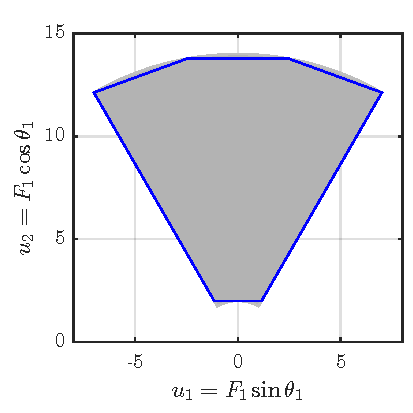
\includegraphics[]{Bicopter/BicopterInputConstraintApprox.pdf}
 \caption{Approximation of the Bicopter input constraints}
 \label{fig:BicopterInputConstraintApprox}
\end{figure}

% acceleration constraint
% \begin{align}
%  \vxd + \wy\vz - \wz\vy + \epsX \big(\wyd + \tfrac{\Jx-\Jz}{\Jy}\wx\wz\big) + \Rzx \gravityAccConst &= 0,
% \\
%  \vyd + \wz\vx - \wx\vz - \epsY \big(\wxd + \tfrac{\Jz-\Jy}{\Jx}\wy\wz\big) + \Rzy \gravityAccConst &= 0,
% \end{align}

\paragraph{Closed loop template.}
Mechanically the bicopter is just a free rigid body, so the control template from \fixme{(??)} is reasonable.
Due to symmetry of the mechanical model we set the center of mass on the body fixed vertical axis and set the principle axis of inertia to be parallel to the body fixed axis, i.e.\ $\scx=\scy=0$ and $\Jc=\diag(\Jcx, \Jcy, \Jcz)$ and the same for damping and stiffness.

\paragraph{Matching}
\begin{align}
 \sysInputMatLComp = \begin{bmatrix} \PropPosZ & 0 & 0 & 0 & -1 & 0 \\ 0 & \PropPosY\cos\PropInc-\PropPosZ\sin\PropInc & 0 & \sin\PropInc & 0 & 0 \end{bmatrix}
\end{align}

constraints on parameters
\begin{align} 
 \lcz &= \hcz,
\\
 \Jcx &= \mc (\hcz-\scz)(\scz-\epsy),&
 \sigcx &= 0,&
 \kapcx &= \mc \gravityAccConst (\hcz-\scz),
\\
 \Jcy &= \mc(\hcz-\scz) (\scz-\epsx),&
 \sigcy &= 0,&
 \kapcy &= \mc \gravityAccConst (\hcz-\scz).
\end{align}
where
\begin{align}
 \epsx = -\tfrac{\Jy}{\m \PropPosZ},
\qquad
 \epsy = \tfrac{\Jx \sin\PropInc}{\m (\PropPosY \cos\PropInc - \PropPosZ \sin\PropInc)}.
\end{align}
This leaves the tuning parameters $\mc, \dc, \kc, \scz, \hcz$ and $\Jcz, \sigcz, \kapcz$.

The remaining matching force is
\begin{align}
 \tilde{\genForce} = 
 \begin{bmatrix} 1 & 0 \\ 0 & 1 \\ 0 & 0 \\ 0 & -\epsy \\ \epsx & 0 \\ 0 & 0 \end{bmatrix}
 \begin{bmatrix}[2]
  \frac{1}{\hcz-\epsx} \big( \Jcz - \mc(\hcz-\scz) (\tfrac{\Jx-\Jz}{\Jy}\epsx - \epsy) \wx\wz - \tfrac{\kapcz}{2}(\Rxz+\Rzx) \big) \\
  \frac{1}{\hcz-\epsy} \big( \Jcz - \mc(\hcz-\scz) (\tfrac{\Jy-\Jz}{\Jx}\epsy - \epsx) \wx\wz - \tfrac{\kapcz}{2}(\Ryz+\Rzy) \big)
%   \frac{\Jcz - \mc(\hcz-\scz) \big(\tfrac{\Jx-\Jz}{\Jy}\epsx - \epsy\big)}{\hcz-\epsx} \wx\wz - \tfrac{\kapcz}{2(\hcz-\epsx)}(\Rxz+\Rzx) \\
%   \frac{\Jcz - \mc(\hcz-\scz) \big(\tfrac{\Jy-\Jz}{\Jx}\epsy - \epsx\big)}{\hcz-\epsy} \wx\wz - \tfrac{\kapcz}{2(\hcz-\epsy)}(\Ryz+\Rzy)
 \end{bmatrix}
\end{align}

\paragraph{Simulation result.}

\begin{figure}[ht]
 \centering
 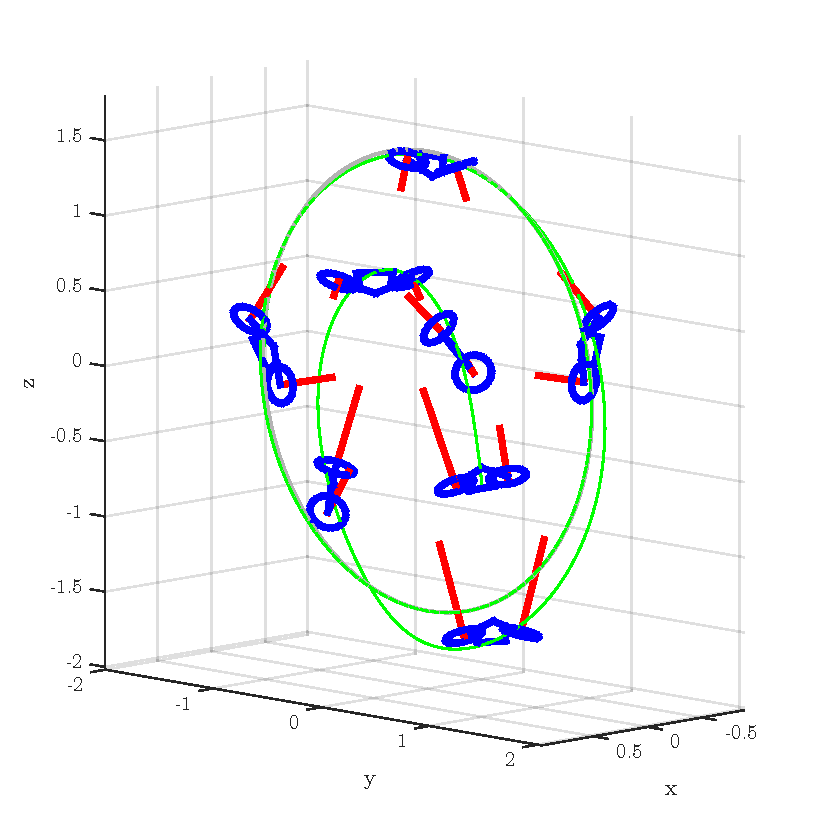
\includegraphics[]{Bicopter/BicopterCircleSimSnapshots.pdf}
 \caption{Simulation result for the Bicopter}
 \label{fig:BicopterCircleSimSnapshots}
\end{figure}

\begin{figure}[p]
 \centering
 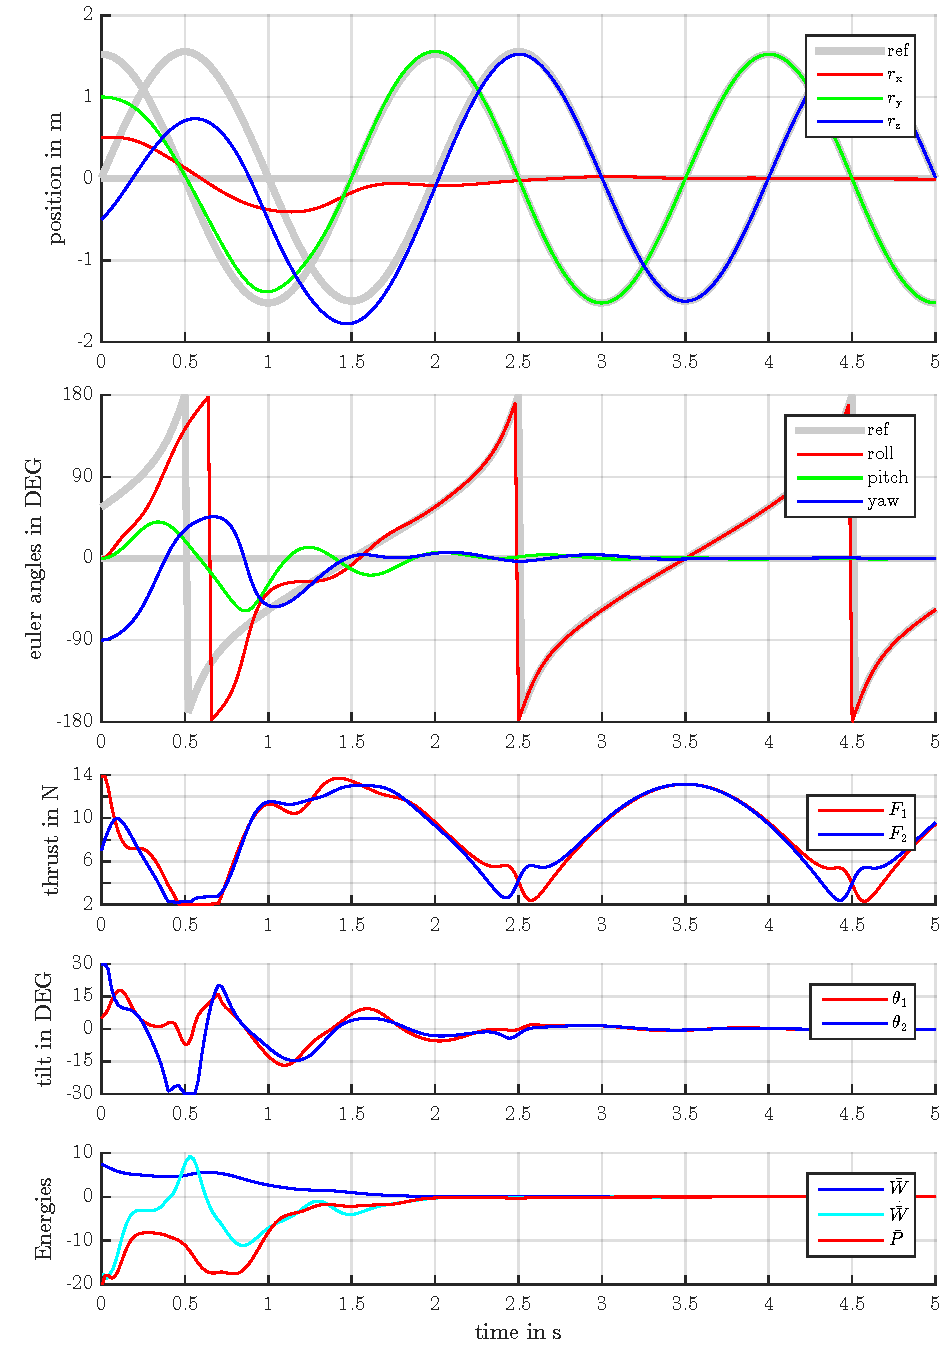
\includegraphics[]{Bicopter/BicopterCircleSimRes.pdf}
 \caption{Simulation result for the Bicopter}
 \label{fig:BicopterCircleSimRes}
\end{figure}
